\title{Neural Networks - Homework 2}
\author{Ryan Spangler}
\date{\today}

\documentclass[12pt]{article}

\usepackage{commath}
\usepackage{graphicx}
\usepackage{listings}
\usepackage{amsfonts}

% python highlighting ----------
\usepackage{color}
\usepackage{listings}
\usepackage{textcomp}
\usepackage{setspace}
%\usepackage{palatino}

\renewcommand{\lstlistlistingname}{Code Listings}
\renewcommand{\lstlistingname}{Code Listing}
\definecolor{gray}{gray}{0.6}
\definecolor{green}{rgb}{0.1,0.6,0.3}
\definecolor{orange}{rgb}{0.9,0.7,0.1}
\definecolor{blue}{rgb}{0,0.6,0.8}

\lstnewenvironment{python}[1][]{
\lstset{
language=python,
basicstyle=\ttfamily\footnotesize\setstretch{1},
stringstyle=\color{red},
showstringspaces=false,
alsoletter={1234567890},
otherkeywords={\ , \}, \{},
keywordstyle=\color{blue},
emph={access,and,break,class,continue,def,del,elif,else,%
except,exec,finally,for,from,global,if,import,in,is,%
lambda,not,or,pass,print,raise,return,try,while},
emphstyle=\color{gray}\bfseries,
emph={[2]True, False, None, self},
emphstyle=[2]\color{orange},
emph={[3]from, import, as},
emphstyle=[3]\color{blue},
upquote=true,
morecomment=[s]{"""}{"""},
commentstyle=\color{gray}\slshape,
emph={[4]1, 2, 3, 4, 5, 6, 7, 8, 9, 0},
emphstyle=[4]\color{blue},
literate=*{:}{{\textcolor{blue}:}}{1}%
	{=}{{\textcolor{blue}=}}{1}%
	{-}{{\textcolor{blue}-}}{1}%
	{+}{{\textcolor{blue}+}}{1}%
	{*}{{\textcolor{blue}*}}{1}%
	{!}{{\textcolor{blue}!}}{1}%
	{(}{{\textcolor{blue}(}}{1}%
	{)}{{\textcolor{blue})}}{1}%
	{[}{{\textcolor{blue}[}}{1}%
	{]}{{\textcolor{blue}]}}{1}%
	{<}{{\textcolor{blue}<}}{1}%
	{>}{{\textcolor{blue}>}}{1},%
    frame=fullbox, rulesepcolor=\color{gray},#1
%framexleftmargin=1mm, framextopmargin=1mm, frame=shadowbox, rulesepcolor=\color{blue},#1
}}{}

\setcounter{secnumdepth}{0}

\begin{document}
\maketitle

\section{Bi-directional Associative Memory}

\subsection{Problem Statement}

The focus of this assignment is to examine the properties, capabilities and limitations of the BAM (Bi-directional Associative Memory), as implemented by NeuralWare.  

\subsection{Experimental Process}

NeuralWare ships with an sample configuration of the BAM mapping a 5x5 pixel grid to a 5x4 pixel grid.  It provides three pairs of trained associations between a 5x5 image and a 5x4 one.  A diagram of these default associations are provided below.  

Since these pairs were already pre-trained, I performed recall on the given patterns.  On the first I added noise to the input pattern (an X) but left the output pattern clean.  For the second that was reversed, and I toggled many bits in the 5x4 grid until seemingly no similarities remained.  For the third I added some noise to both.  In all cases the pattern was restored. 

To test the limits I distorted both sides dramatically, and indeed it did fall into another pattern.  This was often hard to achieve though.  The learned associations were remarkably persistent.

After that I started training new associations to see what the limit of the network was and how many patterns it could reasonably retain without getting overwhelmed and producing false matches.  

\begin{center}
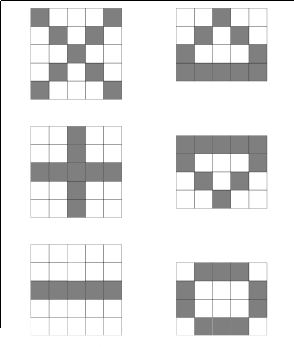
\includegraphics[scale=0.3]{default.png}
\end{center}

\subsection{Results}

It seems if one side of the signal was clear, the other would be restored no matter how noisy it was.  It could be unrecognizable and the integrity of the first was enough to restore the original association.  If both became too noisy it could fall into another pattern, but in the end the association was remarkably robust.  Both patterns could be diverged dramatically and retain enough cues for the algorithm to restore them faithfully.

Once the pattern matched the inverted version of the 5x4 grid, which was predicted in the book.  It seems that if there is more pixels that are on than off, it tends to gravitate towards the inverse pattern.

When training new patterns I noticed the performance really depended on the distinctness of the trained associations.  For instance, a square instead of a circle in the 5x4 pattern (basically with the corners filled in), would produce false matches with the circle pattern under less noise if it and the corresponding 5x5 grid were made increasingly noisy.  

After 4 or 5 new patterns (provided they were sufficiently distinct) the network was surprisingly stable and found correct matches most of the time.  But for the most part beyond that performance suffered.  Beyond getting false matches, the grids would only partially complete patterns before getting stuck, refusing to budge out of incomplete configurations.  It seems the energy minimization function of the network breaks down when too many superimposed association vectors are trained at once.  

Further study could quantify the link between the size of the grids, the number of trained patterns and some kind of distinctness measure between the patterns (possibly just subtraction or a distance measure).  This would provide more insight into the applicability and ultimate usefulness of the BAM network model for real-world applications.

\end{document}  

